\chapter{Architettura del software}
\label{cap:architettura}

\begin{inbreve}
Per costruire un buon prodotto bisogna curare la sua organizzazione complessiva. Il capitolo definisce
l'architettura software e i suoi componenti e elenca gli attributi di qualità non funzionali che essa deve
garantire. Poi tratta in ordine tre temi. Il primo è la decomposizione del sistema, con gli strati e le
preoccupazioni trasversali. Il secondo è l'architettura di distribuzione (client-server, MVC, multi-tier, orientata
ai servizi). Il terzo sono le scelte tecnologiche che vincolano il resto. Le architetture per il cloud sono riprese
nei capitoli~\ref{cap:cloud} e~\ref{cap:microservizi}.
\end{inbreve}

\section{Architettura e componenti}
\label{sec:arch-componenti}

\begin{definizione}[Software architecture, definizione IEEE]
L'architettura è l'organizzazione fondamentale di un sistema software, incorporata nei suoi componenti, nelle loro
relazioni reciproche e con l'ambiente, e nei principi che guidano il suo design e la sua evoluzione.
\end{definizione}

L'architettura influisce su prestazioni, usabilità, sicurezza, affidabilità, manutenibilità e altri attributi del
prodotto.

\begin{definizione}[Component]
Un \termine{componente} è un elemento che implementa un insieme coerente di feature. È una raccolta di
\termine{servizi} che altri componenti possono usare.
\end{definizione}

I servizi di un componente possono essere usati direttamente da altri componenti, oppure solo attraverso
l'\termine{API} del componente (\figrif{fig:arch-componenti}).

\begin{figure}[ht]
\centering
\begin{tikzpicture}[s/.style={draw, minimum width=0.9cm, minimum height=0.7cm, font=\small}]
% componente 1
\node[draw, minimum width=4cm, minimum height=1.6cm] (c1) at (0,0) {};
\node[s] (s1) at (-1.2,0) {S1};
\node[s] (s2) at (0,0) {S2};
\node[s] (s3) at (1.2,0) {S3};
\foreach \n in {s1,s2,s3} \draw[->] ($(\n.north)+(0,1.1)$) -- (\n.north);
\node[font=\footnotesize, align=center] at (0,2.2) {Servizi usati direttamente\\da altri componenti};
\node[font=\small] at (0,-1.2) {Component 1};
% componente 2
\node[draw, minimum width=4cm, minimum height=1.6cm] (c2) at (7,0) {};
\node[s] (s4) at (5.8,0) {S4};
\node[s] (s5) at (7,0) {S5};
\node[s] (s6) at (8.2,0) {S6};
\node[draw, minimum width=4cm, minimum height=0.7cm, font=\small] (api) at (7,1.55) {API};
\foreach \n in {s4,s5,s6} \draw[->] (\n |- api.south) -- (\n.north);
\foreach \x in {5.8,7,8.2} \draw[->] (\x,2.7) -- (\x,1.9);
\node[font=\footnotesize, align=center] at (7,3.3) {Servizi usati attraverso\\l'API del componente};
\node[font=\small] at (7,-1.2) {Component 2};
\end{tikzpicture}
\caption{Due modi di accedere ai servizi di un componente. A sinistra S1, S2 e S3 sono usati direttamente. A destra
S4, S5 e S6 sono raggiungibili solo attraverso l'API.}
\label{fig:arch-componenti}
\end{figure}

\subsection{Che cosa influenza l'architettura}

Cinque fattori influenzano le scelte architetturali.

\begin{description}[leftmargin=0pt, style=unboxed]
  \item[Non-functional product characteristics.] Caratteristiche come sicurezza e prestazioni riguardano tutti gli
    utenti. Se sono sbagliate, il prodotto difficilmente avrà successo commerciale. Alcune sono in contrasto tra loro,
    quindi si può ottimizzare solo la più importante (\rif{sec:arch-nonfunzionali}).
  \item[Product lifetime.] Se si prevede una lunga vita del prodotto, servono revisioni regolari. L'architettura deve
    quindi poter evolvere per accogliere nuove feature e nuove tecnologie.
  \item[Software compatibility.] Per alcuni prodotti è importante la compatibilità con altro software, perché gli
    utenti possano adottare il prodotto e usare dati preparati con un sistema diverso. Questo può limitare le scelte
    architetturali, per esempio il database.
  \item[Number of users.] Se il software per consumatori è distribuito su Internet, il numero di utenti può cambiare
    molto in fretta. Può degradare gravemente le prestazioni, a meno che l'architettura permetta di scalare
    rapidamente il sistema in aumento e in diminuzione.
  \item[Software reuse.] Riutilizzare grandi componenti di altri prodotti o software open source fa risparmiare
    molto tempo e lavoro. Però vincola le scelte architetturali, perché il design deve adattarsi al software riusato.
\end{description}

\section{Attributi di qualità non funzionali}
\label{sec:arch-nonfunzionali}

Gli attributi non funzionali sono importanti per il prodotto finale, non per il prototipo (\rif{sec:prodotti-prototipo}).

\begin{table}[ht]
\centering
\small
\caption{Attributi di qualità non funzionali e domanda chiave associata.}
\label{tab:arch-nonfunzionali}
\begin{tabularx}{\linewidth}{>{\raggedright\arraybackslash}p{3.2cm}X}
\toprule
Attributo & Domanda chiave \\
\midrule
Responsiveness & Il sistema restituisce i risultati agli utenti in un tempo ragionevole? \\
Reliability & Le feature si comportano come si aspettano sia gli sviluppatori sia gli utenti? \\
Availability & Il sistema fornisce i servizi quando gli utenti li richiedono? \\
Security & Il sistema protegge se stesso e i dati degli utenti da attacchi e intrusioni non autorizzati? \\
Usability & Gli utenti accedono alle feature di cui hanno bisogno e le usano in fretta e senza errori? \\
Maintainability & Il sistema si può aggiornare facilmente e si possono aggiungere feature senza costi eccessivi? \\
Resilience & Il sistema continua a fornire servizi agli utenti in caso di guasto parziale o di attacco esterno? \\
\bottomrule
\end{tabularx}
\end{table}

\begin{attenzione}[Compromessi]
Ottimizzare un attributo non funzionale influisce sugli altri. Per esempio, la sicurezza si contrappone a prestazioni e
usabilità. La disponibilità si contrappone a time-to-market e semplicità.
\end{attenzione}

\section{Decomposizione del sistema}
\label{sec:arch-decomposizione}

\begin{definizione}[Service, component, module]
\begin{itemize}
  \item \textbf{Service}: unità coerente di funzionalità.
  \item \textbf{Component}: unità software che offre uno o più servizi.
  \item \textbf{Module}: insieme di componenti.
\end{itemize}
\end{definizione}

Due componenti possono essere in relazione in quattro modi (\figrif{fig:arch-relazioni}):
\begin{itemize}
  \item \emph{is-part-of}: C1 è parte di C2;
  \item \emph{uses}: C1 chiama C2;
  \item \emph{is-located-with}: C1 e C2 si trovano insieme;
  \item \emph{shares-data-with}: C1 e C2 condividono dati.
\end{itemize}

\begin{figure}[ht]
\centering
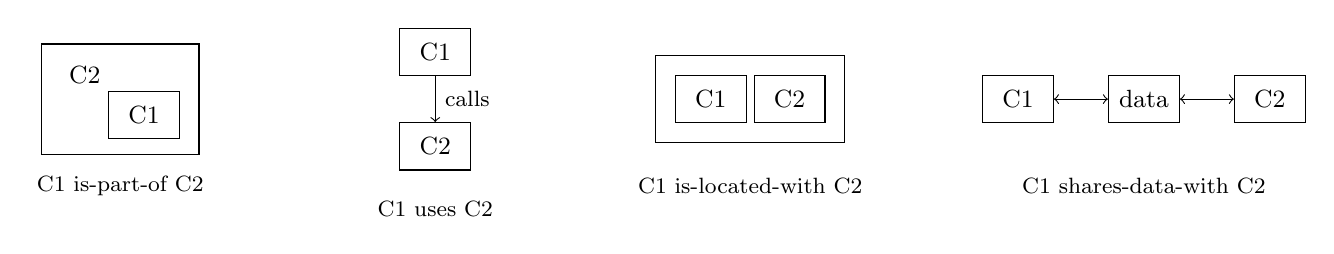
\begin{tikzpicture}[b/.style={draw, minimum width=0.9cm, minimum height=0.6cm, font=\small}]
% is-part-of
\node[draw, minimum width=2cm, minimum height=1.4cm] at (0,0) {};
\node[font=\small] at (-0.45,0.3) {C2};
\node[b] at (0.3,-0.2) {C1};
\node[font=\footnotesize] at (0,-1.1) {C1 is-part-of C2};
% uses
\node[b] (u1) at (4,0.6) {C1};
\node[b] (u2) at (4,-0.6) {C2};
\draw[->] (u1) -- node[right, font=\footnotesize] {calls} (u2);
\node[font=\footnotesize] at (4,-1.4) {C1 uses C2};
% is-located-with
\node[draw, minimum width=2.4cm, minimum height=1.1cm] at (8,0) {};
\node[b] at (7.5,0) {C1};
\node[b] at (8.5,0) {C2};
\node[font=\footnotesize] at (8,-1.1) {C1 is-located-with C2};
% shares-data-with
\node[b] (d1) at (11.4,0) {C1};
\node[b] (dd) at (13,0) {data};
\node[b] (d2) at (14.6,0) {C2};
\draw[<->] (d1) -- (dd);
\draw[<->] (dd) -- (d2);
\node[font=\footnotesize] at (13,-1.1) {C1 shares-data-with C2};
\end{tikzpicture}
\caption{Le quattro relazioni possibili tra componenti.}
\label{fig:arch-relazioni}
\end{figure}

\begin{attenzione}[Complessità]
Man mano che il numero di componenti cresce, il numero di relazioni tende a crescere \emph{più in fretta}. La
semplicità è essenziale (manifesto agile, \rif{sec:agile-manifesto}).
\end{attenzione}

Per controllare la complessità ci sono tre linee guida:
\begin{itemize}
  \item \textbf{Separation of concerns}: organizzare l'architettura in componenti ciascuno concentrato su una sola
    preoccupazione (\ingl{concern});
  \item \textbf{Stable interfaces}: progettare interfacce di componente coerenti, che cambiano lentamente;
  \item \textbf{Implement once}: evitare di duplicare la stessa funzionalità in punti diversi dell'architettura.
\end{itemize}

\section{Architetture a strati}
\label{sec:arch-strati}

Un'\termine{architettura a strati} (\ingl{layered}) organizza il sistema così:
\begin{itemize}
  \item ogni strato è un'area di interesse (\ingl{concern}) ed è considerato separatamente dagli altri;
  \item dentro uno strato i componenti sono indipendenti e non si sovrappongono nelle funzionalità;
  \item il modello è di alto livello e non contiene informazioni di implementazione.
\end{itemize}
Nella pratica le preoccupazioni non sono sempre separate al 100\%. Nell'esempio di \figrif{fig:arch-strati} la
validazione compare in due strati: nel browser (\emph{local input validation}) e nei servizi di base
(\emph{query validation}), sottolineati in figura.

\begin{figure}[ht]
\centering
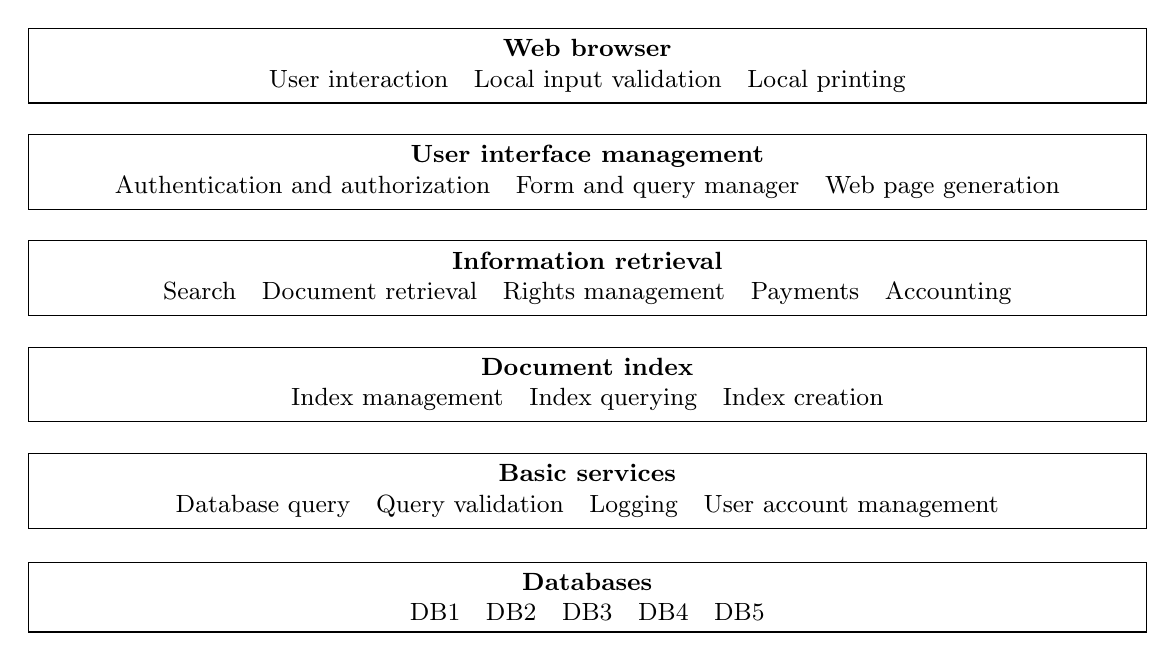
\begin{tikzpicture}[st/.style={draw, minimum width=14.2cm, align=center, font=\small, inner sep=4pt}]
\node[st] (a) at (0,0) {\textbf{Web browser}\\User interaction\quad\uline{Local input validation}\quad Local printing};
\node[st] (b) at (0,-1.35) {\textbf{User interface management}\\Authentication and authorization\quad Form and query manager\quad Web page generation};
\node[st] (c) at (0,-2.7) {\textbf{Information retrieval}\\Search\quad Document retrieval\quad Rights management\quad Payments\quad Accounting};
\node[st] (d) at (0,-4.05) {\textbf{Document index}\\Index management\quad Index querying\quad Index creation};
\node[st] (e) at (0,-5.4) {\textbf{Basic services}\\Database query\quad \uline{Query validation}\quad Logging\quad User account management};
\node[st] (f) at (0,-6.75) {\textbf{Databases}\\DB1\quad DB2\quad DB3\quad DB4\quad DB5};
\end{tikzpicture}
\caption{Esempio di architettura a strati di un sistema di recupero di documenti. Dall'alto: browser, gestione
dell'interfaccia, recupero delle informazioni, indice dei documenti, servizi di base, database. Sono sottolineati i
due componenti di validazione, presenti in strati diversi.}
\label{fig:arch-strati}
\end{figure}

\subsection{Cross-cutting concerns}

Le \termine{cross-cutting concerns} sono preoccupazioni di sistema che riguardano l'intero sistema, per esempio
sicurezza, prestazioni e affidabilità (\figrif{fig:arch-trasversali}). Ogni strato deve tenerne conto, quindi esse
\emph{aggiungono interazioni tra gli strati}.

\begin{figure}[ht]
\centering
\begin{tikzpicture}
\foreach \y/\n in {0/User interface, -0.65/Application, -1.3/Infrastructure, -1.95/Operating system, -2.6/Hardware} {
  \draw (-4.5,\y-0.3) rectangle (4.5,\y+0.3);
  \node[font=\small, anchor=west] at (-4.4,\y) {\n};
}
\foreach \x/\n in {0.4/Security, 2.1/Performance, 3.8/Reliability} {
  \draw[->, very thick, blu] (\x,1.1) -- (\x,-3.1);
  \node[font=\footnotesize\sffamily, fill=white, inner sep=1pt] at (\x,1.35) {\n};
}
\end{tikzpicture}
\caption{Le preoccupazioni trasversali (security, performance, reliability) attraversano tutti gli strati del sistema.}
\label{fig:arch-trasversali}
\end{figure}

\begin{esempio}[Security architecture]
Strati diversi usano tecnologie diverse, per esempio un database SQL o il browser Firefox. Gli attaccanti possono
sfruttarne le vulnerabilità per ottenere l'accesso. Serve quindi protezione da attacchi a ogni strato e anche
protezione dagli attacchi già riusciti agli strati superiori. Se c'è un solo componente di sicurezza, esso è una
vulnerabilità critica. Tutti i controlli passano da quel componente: se smette di funzionare, o è compromesso, il
sistema non ha più sicurezza affidabile. Distribuire la sicurezza tra gli strati rende il sistema più resistente agli
attacchi e ai guasti del software.
\end{esempio}

\subsection{Strati generici per un'applicazione web}

\begin{table}[!ht]
\centering
\small
\caption{Strati generici di un'applicazione web. L'architetto personalizza questo schema decidendo se servono più o
meno strati.}
\label{tab:arch-strati-web}
\begin{tabularx}{\linewidth}{>{\raggedright\arraybackslash}p{4cm}X}
\toprule
Strato & Spiegazione \\
\midrule
Browser-based or mobile user interface & Interfaccia di sistema in un browser web in cui spesso si usano form HTML per
  raccogliere l'input. A questo livello vanno incluse anche componenti JavaScript per azioni locali, come la
  validazione dell'input. In alternativa l'interfaccia mobile può essere un'app. \\
Authentication and UI management & Strato di gestione dell'interfaccia utente che può includere componenti per
  l'autenticazione degli utenti e la generazione delle pagine web. \\
Application-specific functionality & Strato ``applicazione'' che offre le funzionalità specifiche dell'applicazione.
  A volte si suddivide in più strati. \\
Basic shared services & Strato di servizi condivisi con componenti che offrono servizi usati dallo strato
  applicazione. \\
Database and transaction management & Strato di database che offre servizi come la gestione delle transazioni e il
  recovery. Se l'applicazione non usa un database, può non servire. \\
\bottomrule
\end{tabularx}
\end{table}

\begin{attenzione}[Decomposizione e tecnologie]
La decomposizione del sistema va fatta, in parte, insieme alla scelta delle tecnologie. Per esempio, scegliere un
database relazionale condiziona i componenti agli strati più alti. Scegliere di supportare interfacce su dispositivi
mobili richiede i relativi toolkit di sviluppo dell'interfaccia (\rif{sec:arch-tecnologie}).
\end{attenzione}

\section{Architettura di distribuzione}
\label{sec:arch-distribuzione}

L'\termine{architettura di distribuzione} definisce i server e l'assegnazione dei componenti ai server.

\subsection{Client-server}

L'architettura \termine{client-server} è adatta alle applicazioni in cui i client accedono a un database condiviso e a
operazioni di logica di business su quei dati. Ci sono più server (per esempio web server e database server) con
bilanciamento del carico (\figrif{fig:arch-clientserver}).

\begin{figure}[ht]
\centering
\begin{tikzpicture}[cl/.style={draw, ellipse, minimum width=1.6cm, minimum height=0.7cm, font=\small}]
\foreach \i/\y in {1/1.8, 2/0.6, 3/-0.6} \node[cl] (c\i) at (0,\y) {Client \i};
\node[cl] (c4) at (0,-1.8) {Client \dots};
\node[draw, minimum width=0.5cm, minimum height=4cm] (lb) at (3.6,0) {};
\node[font=\footnotesize, align=center] at (3.6,-2.6) {Load\\balancer};
\node[draw, minimum width=2.6cm, minimum height=1.8cm] (sv) at (7,0) {};
\foreach \x in {6.3,7,7.7} \foreach \y in {0.4,-0.4} \node[draw, fill=grigiochiaro, minimum size=0.45cm] at (\x,\y) {};
\node[font=\footnotesize] at (7,-1.4) {Servers};
\foreach \i in {1,2,3,4} \draw[<->] (c\i) -- (lb.west |- c\i);
\draw[<->] (lb.east) -- (sv.west);
\end{tikzpicture}
\caption{Architettura client-server. Molti client inviano richieste e ricevono risposte da un insieme di server,
attraverso un bilanciatore del carico (\ingl{load balancer}) che le distribuisce.}
\label{fig:arch-clientserver}
\end{figure}

\subsubsection{Il pattern Model-View-Controller}
Il pattern \termine{Model-View-Controller} (MVC) è un pattern architetturale per l'interazione client-server
(\figrif{fig:arch-mvc}):
\begin{itemize}
  \item il modello (\emph{model}) è disaccoppiato dalla sua presentazione;
  \item ogni vista (\emph{view}) si registra presso il modello, così che se il modello cambia tutte le viste possano
    essere aggiornate.
\end{itemize}

\begin{figure}[ht]
\centering
\begin{tikzpicture}[o/.style={draw, ellipse, minimum width=2cm, minimum height=0.8cm, font=\small}]
\draw (-0.2,0.9) rectangle (9.2,4.4);
\node[font=\footnotesize\sffamily] at (0.6,4.1) {CLIENT};
\draw (2.4,-2.6) rectangle (6.8,-0.9);
\node[font=\footnotesize\sffamily] at (3.4,-2.3) {SERVER};
\node[o] (br) at (4.5,3.7) {Browser};
\node[o] (co) at (1.9,1.5) {Controller};
\node[o] (vi) at (7.1,1.5) {View};
\node[o] (mo) at (4.5,-1.75) {Model};
\draw[->] (br) -- node[left, font=\footnotesize] {user inputs} (co);
\draw[->] (vi) -- node[right, font=\footnotesize] {page to display} (br);
\draw[->] (vi) -- node[above, font=\footnotesize] {user changes} (co);
\draw[->] (co) -- node[left, font=\footnotesize, align=right] {view update\\request} (mo);
\draw[->] (mo) -- node[right, font=\footnotesize, align=left] {change\\notification} (vi);
\end{tikzpicture}
\caption{Il pattern MVC nell'interazione client-server. Sul client il Browser passa l'input utente al Controller, che
chiede un aggiornamento al Model sul server. Il Model notifica il cambiamento alla View, che invia al Browser la
pagina da mostrare. Le modifiche dell'utente nella View sono comunicate al Controller.}
\label{fig:arch-mvc}
\end{figure}

\begin{esempio}[MVC in un negozio online\aggiunta]
Il \emph{model} contiene il carrello, sul server. Le \emph{view} sono la pagina del carrello e l'icona con il numero
di articoli. Quando l'utente preme ``aggiungi'', il \emph{controller} riceve l'azione e chiede al model di aggiungere
l'articolo. Il model cambia e notifica tutte le view registrate: la pagina e l'icona si aggiornano insieme. Il model
non sa come sono disegnate le view, quindi se ne può aggiungere una nuova (per esempio un'app mobile) senza toccarlo.
\end{esempio}

\subsection{Multi-tier e orientata ai servizi}

La comunicazione client-server avviene di solito con HTTP e con dati in XML o JSON. Esistono due varianti
(\figrif{fig:arch-tier}):
\begin{itemize}
  \item \termine{multi-tier}: il web server comunica con un application server, che comunica con il database
    server;
  \item \termine{service-oriented architecture} (SOA): il web server comunica con un service gateway che dà accesso a
    un insieme di servizi indipendenti (s1, \dots, s6).
\end{itemize}

\begin{figure}[ht]
\centering
\begin{tikzpicture}[b/.style={draw, minimum width=1.9cm, minimum height=0.8cm, font=\small, align=center},
  cl/.style={draw, ellipse, minimum width=1.2cm, font=\footnotesize}]
\node[font=\small\bfseries\sffamily] at (-3.2,1.7) {Multi-tier};
\node[cl] (c1) at (-3.2,0.9) {Client};
\node[cl] (c2) at (-3.2,-0.1) {Client};
\node[b] (w) at (0,0.4) {Web\\server};
\node[b] (ap) at (3,0.4) {Application\\server};
\node[b] (db) at (6,0.4) {Database\\server};
\draw[<->] (c1) -- (w); \draw[<->] (c2) -- (w);
\draw[<->, thick] (w) -- (ap); \draw[<->, thick] (ap) -- (db);
\node[font=\small\bfseries\sffamily] at (-3.2,-2.0) {Service-oriented};
\node[cl] (d1) at (-3.2,-2.8) {Client};
\node[cl] (d2) at (-3.2,-3.8) {Client};
\node[b] (w2) at (0,-3.3) {Web\\server};
\node[b] (g) at (3,-3.3) {Service\\gateway};
\draw[<->] (d1) -- (w2); \draw[<->] (d2) -- (w2);
\draw[<->, thick] (w2) -- (g);
\foreach \i/\y in {1/-1.9, 2/-2.5, 3/-3.1, 4/-3.7, 5/-4.3, 6/-4.9} {
  \node[draw, minimum size=0.5cm, font=\footnotesize] (s\i) at (6,\y) {s\i};
  \draw[<->] (g.east) -- (s\i.west);
}
\end{tikzpicture}
\caption{In alto: architettura multi-tier. In basso: architettura orientata ai servizi, con un gateway che dà accesso
ai servizi s1--s6.}
\label{fig:arch-tier}
\end{figure}

\subsection{Come scegliere l'architettura di distribuzione}

\begin{description}[leftmargin=0pt, style=unboxed]
  \item[Data type and data updates.] Se i dati sono per lo più strutturati e possono essere aggiornati da feature
    diverse, di solito è meglio un unico database condiviso, che offre locking e gestione delle transazioni. Se i dati
    sono distribuiti tra più servizi, serve un modo per mantenerli coerenti e questo aggiunge overhead.
  \item[Change frequency.] Se si prevede che i componenti siano cambiati o sostituiti con regolarità, isolarli come
    servizi separati semplifica i cambiamenti.
  \item[The system execution platform.] Se il sistema gira sul cloud con utenti che vi accedono via Internet, di solito è
    meglio un'architettura orientata ai servizi, perché scalare è più semplice. Se è un sistema aziendale su server
    locali, può essere più adatta una multi-tier.
\end{description}

\section{Questioni tecnologiche}
\label{sec:arch-tecnologie}

Le scelte tecnologiche influenzano e vincolano l'architettura complessiva. Sono difficili e costose da cambiare
durante lo sviluppo. Le principali riguardano database, piattaforma di consegna, server e tecnologie di sviluppo.

\subsection{Database}

\begin{description}[leftmargin=0pt, style=unboxed]
  \item[Database relazionali] (per esempio MySQL). I dati sono organizzati in tabelle strutturate. Sono adatti soprattutto
    quando servono la gestione delle transazioni e le strutture dati sono prevedibili e semplici.
  \item[Database NoSQL] (per esempio MongoDB). L'organizzazione dei dati è più flessibile e definita dall'utente.
    Sono più flessibili ed efficienti per l'analisi dei dati. I dati possono essere organizzati in modo gerarchico ed
    è possibile l'elaborazione concorrente efficiente dei ``big data''.
\end{description}

\begin{esempio}[Quale database scegliere\aggiunta]
Un registro di conti correnti ha dati con struttura fissa e prevedibile e richiede transazioni: un bonifico deve
sottrarre da un conto e aggiungere all'altro, o fare entrambe le cose o nessuna. È il caso di un database relazionale.
Un servizio che raccoglie i clic di milioni di utenti ha dati dalla forma variabile, da elaborare in parallelo in
grande quantità: è il caso di un database NoSQL.
\end{esempio}

\subsection{Piattaforma di consegna}

Il prodotto può essere consegnato come prodotto web o mobile. Nel mobile i problemi sono:
\begin{itemize}
  \item connettività intermittente;
  \item potenza del processore;
  \item gestione dell'energia;
  \item schermo ridotto e tastiera su schermo.
\end{itemize}
Le versioni web e mobile possono richiedere architetture di decomposizione diverse (per esempio per mantenere le
prestazioni). Quindi bisogna decidere presto se concentrarsi sulla versione mobile o su quella desktop.

\subsection{Server}

Il prodotto può girare sui server dei clienti o sul cloud.
\begin{itemize}
  \item Per i prodotti per consumatori: SOA più cloud.
  \item Per i prodotti aziendali ci possono essere preoccupazioni sulla sicurezza del cloud e meno bisogno di gestire
    picchi di domanda.
  \item Se si sviluppa per il cloud, la decisione successiva è scegliere il fornitore. Spostare il prodotto tra
    fornitori non è facile: è il \termine{vendor lock-in}.
\end{itemize}

\subsection{Tecnologie di sviluppo}

Le tecnologie di sviluppo (per esempio un toolkit di sviluppo mobile o un framework per applicazioni web)
influenzano l'architettura del prodotto. Per esempio, molti framework web presuppongono il pattern MVC. Possono
influenzarla anche indirettamente: se il team è abituato ai database relazionali, tenderà a sceglierne uno.

\begin{puntichiave}
\begin{itemize}
  \item L'architettura è l'organizzazione fondamentale di un sistema: componenti, relazioni, principi di design.
    Influisce su prestazioni, usabilità, sicurezza, affidabilità, manutenibilità.
  \item Un componente offre servizi, usati direttamente o tramite API. Un modulo è un insieme di componenti.
  \item Gli attributi non funzionali (responsiveness, reliability, availability, security, usability,
    maintainability, resilience) si influenzano a vicenda.
  \item Le relazioni crescono più in fretta dei componenti. Linee guida: separation of concerns, stable interfaces,
    implement once.
  \item Architettura a strati; le cross-cutting concerns attraversano tutti gli strati.
  \item Distribuzione: client-server (MVC), multi-tier, SOA. Si sceglie in base a dati, frequenza di cambiamento e
    piattaforma.
  \item Le scelte tecnologiche (database, piattaforma, server, strumenti) vincolano l'architettura e sono costose da
    cambiare.
\end{itemize}
\end{puntichiave}

\begin{domande}
\begin{enumerate}
  \item Che cos'è l'architettura software e quali attributi del prodotto influenza?
  \item Che differenza c'è tra servizio, componente e modulo?
  \item Elencare gli attributi non funzionali e dare un esempio di compromesso tra due di essi.
  \item Perché la complessità cresce più in fretta del numero di componenti? Quali linee guida la controllano?
  \item Che cos'è un'architettura a strati e che cosa sono le cross-cutting concerns?
  \item Che cos'è il pattern MVC?
  \item Come si scelgono la distribuzione del sistema e il database? Quando conviene la SOA?
  \item Che cos'è il vendor lock-in?
\end{enumerate}
\end{domande}
